% author: Tomas Trnka
% mail: tomas@trnkatomas.eu
% date: 2013-07-04

\documentclass[a4paper,10pt]{article}
%\usepackage[czech]{babel}
%\usepackage[T1]{fontenc}
\usepackage[hmargin=2.2cm,vmargin=2.2cm]{geometry}
\usepackage[utf8x]{inputenc}
\usepackage{fancyhdr}
\usepackage{fancyvrb}
\usepackage{amsmath} 
\usepackage{float}
\usepackage{enumerate}
\usepackage{tikz}
\usepackage{hyperref}
\pagestyle{fancy}
\headheight 15pt
\lhead{Crpyto, Fall 2014}
\rhead{Tomas Trnka}
\newcommand{\set}[1]{\ensuremath{\left\lbrace #1 \right\rbrace}}
\newcommand{\role}[1]{\ensuremath{\left\langle #1 \right\rangle}}
\newcommand{\cara}{\begin{center}\rule{140mm}{.2mm}\end{center}}
\newcommand{\mI}{\ensuremath{^\mathcal{I}}}
\newcommand{\Tbox}[1]{\ensuremath{\mathcal{T}}-Box#1}
\newcommand{\Abox}[1]{\ensuremath{\mathcal{A}}-Box#1}
\newcommand{\mC}[1]{\ensuremath{\mathcal{#1}}}
\newcommand{\Tc}{\ensuremath{\mathcal{T}_c}}
\newcommand{\qb}[1]{\ensuremath{\vert{#1}\rangle}}
\begin{document}
\section*{Public-key crypto based on factoring}
This section relies on something called one-way trapdoor fucntions, unfortunately these functions are not proven to be unconditionally secure and therefore the security is concern about only computational security.
\subsection*{RSA}
The basic definition is as follows
\begin{itemize}
\item Gen(K)
\item generate k-bit primes p,q such that n=pq
\item select $e \in N, gcd(e(p-1)(q-1))=1$
\item compute $d = e^{-1} \mod (p-1)(q-1)$
\item than we have public key (n,e), and secret key (n,d)
\item $m \in Z_n E_{pk}(m) = m^e \mod n, D_{sk}(c) = c^d \mod n$
\end{itemize}
Why is this thing working? $c^d \equiv m^{e^d} \equiv m^{ed} \mod n$  according to Euler's totient function, $\varphi(n) = \varphi(p-1)\varphi(q-1)$.
\begin{eqnarray*}
x^{ed} \mod m &\equiv & x^{1 + h\varphi(n)} \mod n\\
x x^{h^{\varphi(n)}} & \equiv & x1 \mod pq\\
\end{eqnarray*}
according to Chinese reminder theorem, the same for the second variable and according to the Chinese reminder theorem 
\begin{eqnarray*}
n &=& pq\\
ab \mod n &=& c\\
gcd(p,q) &=& 1\\
a,b &\in & Z_n\\
(a \mod p&,&a \mod q),(b \mod p,b \mod q)\\
(ab \mod p&,&ab \mod q) = (c \mod p, c \mod q)
\end{eqnarray*}
\begin{eqnarray*}
x^{ed} & \equiv & x^{(ed-1)}x \mod p\\
ed &\equiv & 1 \mod(p-1)(q-1)\\
ed - 1 &\equiv & t(p-1)(q-1) \mod (p-1)(q-1)\\
x^{t(p-1)(q-1)}x & \equiv &  x^{(p-1)^{t(q-1)}}x = x\mod p \text{ Fermat little theorem}\\
\end{eqnarray*}
\begin{itemize}
\item at most secure as factoring $\rightarrow$ polynomial reduction to factoring algorithm	
\item defined by triplet (G,E,D)
\item \textbf{G, algorithm for generating keys:}\\
 This algorithm is probabilistic, takes a security parameter \textit{k} as inout and always outputs a pair of keys \textit{(pk,sk)}, the public and secret keys. We assume
that from the public key one easily derive a description of $\mathcal{P}$, the set of plaintexts and $\mathcal{C}$, the
set of ciphertexts. These do not have to be the same for every key.
set of ciphertexts. These do not have to be the same for every key.
\item 
\textbf{E, algorithm for encryption:} this algorithm takes as input pk and $x \in P$ and produces as
output $E_{pk}(x) \in \mathcal{C}$. Note that \textit{E} may be probabilistic, that is, even though we fix x and K, many
different ciphertexts may be produced as output from E, as a result of random choices made during the encryption process. In other words, the ciphertext will have a probability distribution that is determined from \textit{x} and \textit{K}, typically uniform in some subset of the ciphertexts.
\item
\textbf{D, algorithm for decryption:}\\
this algorithm takes as input $sk,y \in \mathcal{C}$ and produces as output $D_sk(y) \in \mathcal{P}$. It is allowed to be probabilistic, but is in most cases deterministic.
\end{itemize}
\begin{itemize}
\item Trapdoor one-way function -- the principle why this is working
\item the easiest description of RSA:\\
The public encryption key is \textit{pk = (n,e)}, while the secret decryption key is \textit{sk = (n,d)} The
set of plaintexts and the set of ciphertexts are the equal, namely P = C = Zn. And finally, the encryption operation is $E_{pk}(x) = xe \mod n$, while $D_{sk}(y) = yd\mod n$.
\end{itemize}
\textbf{Definition 3.} We will say that the system \textit{(G,E,D)} forms a family of trapdoor one-way functions
if the following is satisfied:
\begin{itemize}
\item
The algorithms \textit{(G,E,D)} defining the system all run in time polynomial in the security parameter \textit{k}.
\item 
Let any probabilistic polynomial time algorithm A be given. Consider the following experiment:
we run G on input k, let (pk,sk) be the output. Then we select x at random in the set of
plaintexts P and finally we run A on input pk,Epk(x), i.e. we give A the public key and the
encryption of a random plaintext. Let p(A,k) be the probability that A outputs x. Then we
require that for any A, p(A,k) is negligible in k.
A probability $\epsilon(k)$ that depends on k is negligible if it holds that for any polynomial f, we have
$\epsilon(k) ≤ 1/f(k)$ for all large enough k. In other words, asymptotically in k, it vanishes to zero
very quickly. This is a complexity theoretic way to say that “for all practical purposes”, the
probability might as well have been zero.
\end{itemize}
Definition of security for such system
\begin{itemize}
\item[] \textbf{The ideal world:}\\
Input to both adversary A and oracle O is the security parameter k. The oracle runs G(k) to get (pk,sk) and gives pk to A. A computes a plaintext x ∈ P and gives it to O. The oracle responds with $E_{pk}(r)$, where r is randomly chosen in P of the same length as x.
Finally A outputs a bit b.

\item[] \textbf{The real world:}\\
Input to both adversary A and oracle O is the security parameter k. The oracle runs G(k) to get (pk,sk) and gives pk to A. A computes a plaintext x ∈ P and gives it to O.
The oracle responds with $E_{pk}(x)$. Finally A outputs a bit b.	
\end{itemize}
We define $p_{A,ideal}(k) (p_{A,real}(k))$ to be the probability that A outputs 1 in the ideal world (the real world) on input k, and the advantage of A to be
$$
Adv_A(k) = |p_{A,ideal}(k) - p_{A,real}(k)|
$$

But since the RSA system is deterministic we clearly can do such think - the adversary can compute everything by itself and the compare to the results.

However, it is possible to use deterministic systems to build new ones that do have this type
of security. Let us take RSA as an example. Let (G,D,E) be the following public-key system: G
simply generates a pair of RSA keys (n,e), (n,d) in the usual way. However, the set of messages
is just {0,1} whereas the set of ciphertexts is $Z^{∗}_n$. The encryption algorithm E will encrypt a bit b
by choosing a random number $x_b \in Z^{∗}_n$ such that the least significant bit of $x_b$ is b. The ciphertext is now $c = x^e_b \mod n$. Decryption is straightforward: reconstruct $x_b$ using the secret RSA key and extract the least significant bit.

\subsection*{Attacks}
Quadratic sieve method - factoring N\\
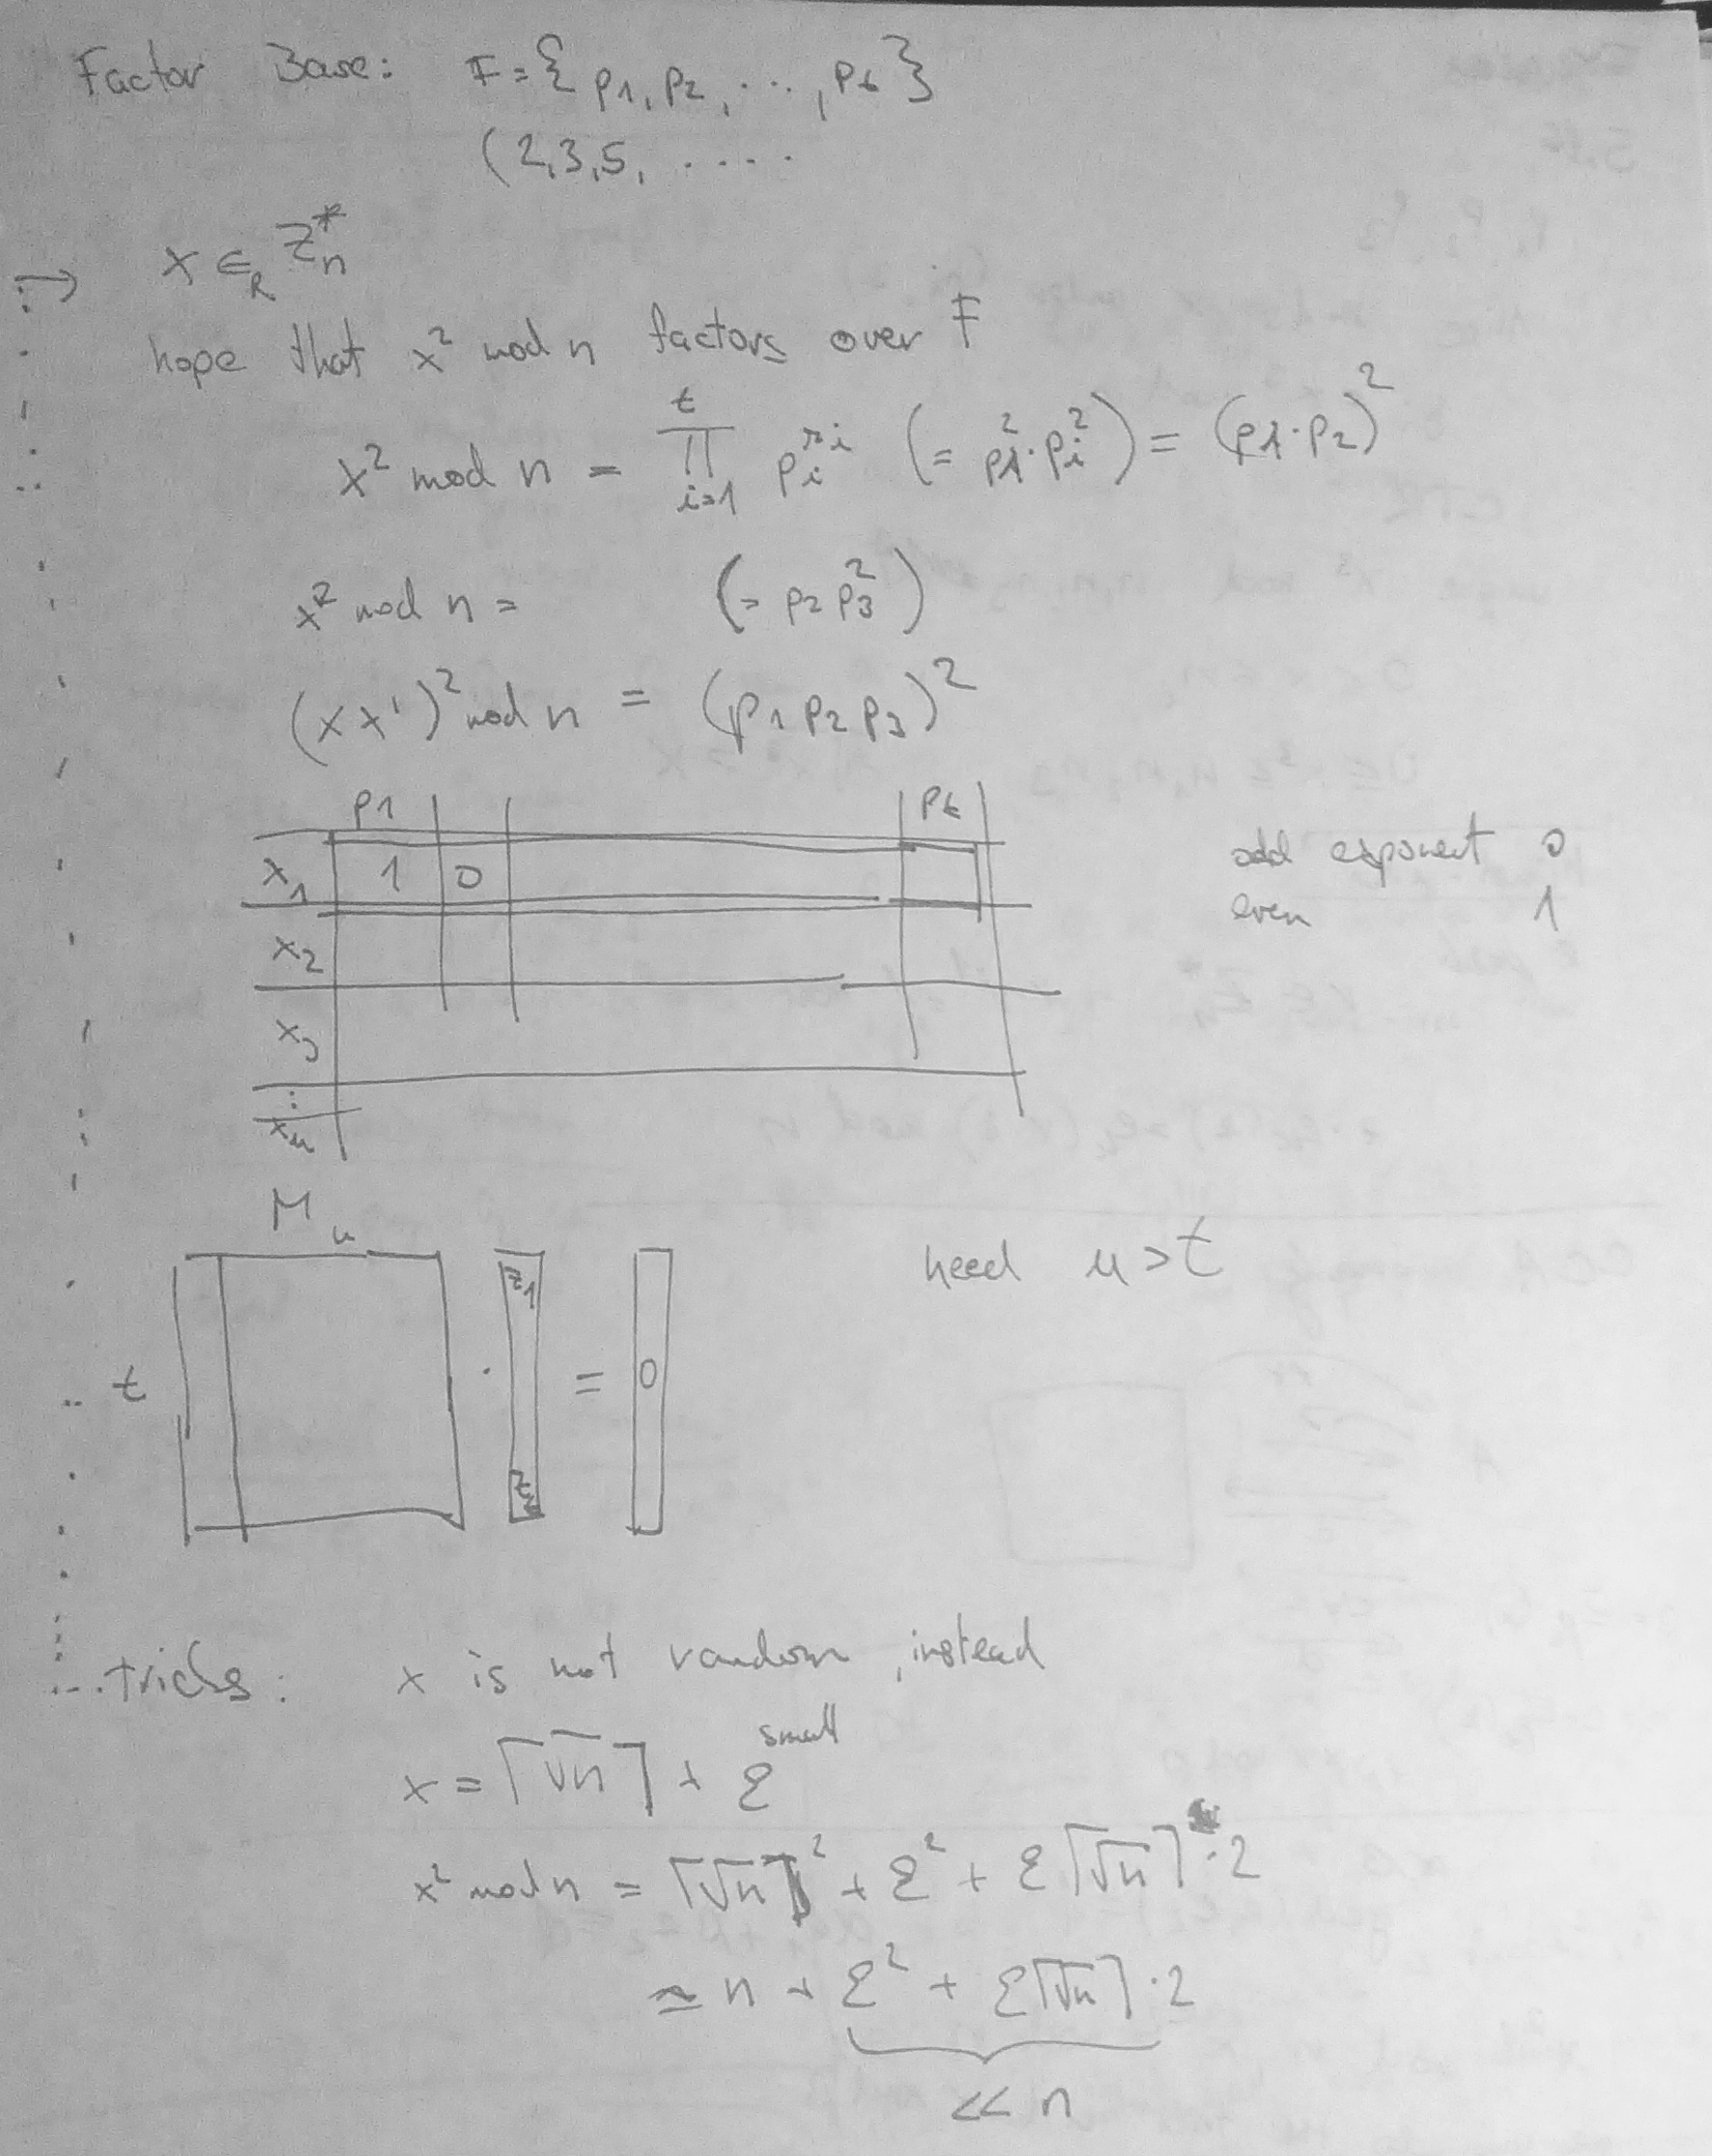
\includegraphics[width=0.5\textwidth]{rsa_attack.jpg}\\
Peter Shor's quantum
Number Field Sieve
Time attacks

\subsection*{Key generation}
To get our cryptosystem working we need to have fairly large prime numbers (in order of thousands bits). 
\subsubsection*{Miller-Rubin primality test}
We test some odd number x
\begin{enumerate}
\item choose $r \in_R Z_x$
\item $gcd(r,x) \neq 1$, reject
\item $x-1 = 2^a\cdot b$, from fermat little theorem $k^{(l-1)} = 1 \mod l$
\item iterate $r^{2b},r^{2^2b},r^{2^3b}$
\item if there is -1 in the list then accept, also $r^b \mod x = 1$ yield accept
\end{enumerate}

\subsection*{Information about certain bits}
One can by dividing $\frac{e_K(x)}{n} = \left(\frac{x}{n}\right)^b = \frac{x}{n}$ obtain parity of the last bit in plain text - therefore OAEP.

\subsection*{Chosen Ciphertext Security}
There are discussions whether we are not giving the adversary too much power - but the reality denies such worries. It was the case for SSL-PCKS\#1. We again have:
\begin{itemize}
\item
\textbf{The ideal world:}\\ Input to both adversary A and oracle O is the security parameter k. The oracle
runs G(k) to get (pk,sk) and gives pk to A. A may now submit an input string y to O, and
O will return Dsk(y) to A. This is repeated as many time as A wants. Then A computes a
plaintext x ∈ P and gives it to O. The oracle responds with y0= Epk(r), where r is randomly
chosen in P of the same length as x. A may now again submit an input string y to O, the only
restriction is that y must be different from y0. O will return Dsk(y) to A. This is repeated as
many time as A wants.Finally A outputs a bit b.
\item
\textbf{The real world:}\\ Input to both adversary A and oracle O is the security parameter k. The oracle
runs G(k) to get (pk,sk) and gives pk to A. A may now submit an input string y to O, and
O will return Dsk(y) to A. This is repeated as many time as A wants. Then A computes a
plaintext x ∈ P and gives it to O. The oracle responds with y0= Epk(x). A may now again
submit an input string y to O, the only restriction is that y must be different from y0. O will
return Dsk(y) to A. This is repeated as many time as A wants.
Finally A outputs a bit b.
\end{itemize}
We define pA,ideal(k),pA,real(k) as for semantic security, and the advantage of A to be
$$Adv_A(k) = |pA,ideal(k) − pA,real(k)|$$
Definition 5. We say that (G,E,D) is chosen ciphertext (CCA)-secure, if for all probabilistic polynomial time adversaries A, it holds that $Adv_A(k)$ is negligible in k.

This unfortunately lead to very inefficient  systems - therefore we will introduce OAEP - Optimal asymmetric encryption padding) - Basic idea of this is map all the strings from large pool P into much smaller P - which give the adversary no additional information.
\begin{enumerate}
\item Choose $r \in {0,1}^{k_0}$ at random.
\item Compute $s = G(r) ⊕ (m||0^{k_1})$, t = H(s) ⊕ r, w = s$||$t, where $||$ means concatenation of strings.
\item  Let the ciphertext be $E_{pk}(w)$.
\end{enumerate}
No method of the OAEP type have been proved secure in the sense that their security follows
only only from the RSA assumption, for instance. The problem is that it seems very difficult to
design the encoding method such that one can prove that it is hard to generate legal ciphertexts
wihtout knowing the plaintext. But they can nevertheless be quite adequate in practice, and OAEP is a part of many international standards for encryption, particularly in connection with RSA.

\end{document}